% !TEX root = ../main.tex

% Background section

\section{Verifying Variational Boosting's Effectiveness} \label{sec:verify}

\begin{figure}[H]
\centering
\begin{subfigure}{0.45\textwidth}
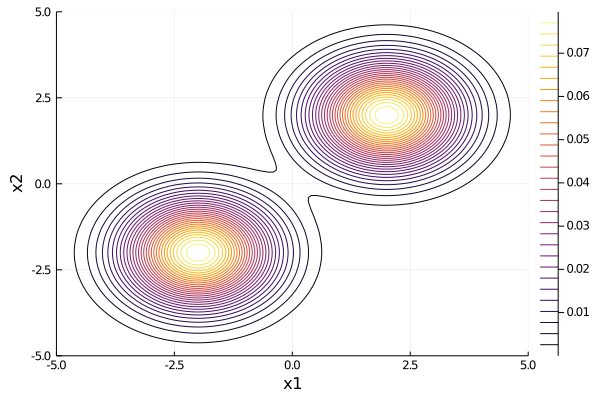
\includegraphics[width=1\linewidth]{../../plot/true_post_far.png}
\caption{True posterior distritbution}
\end{subfigure}
\begin{subfigure}{0.45\textwidth}
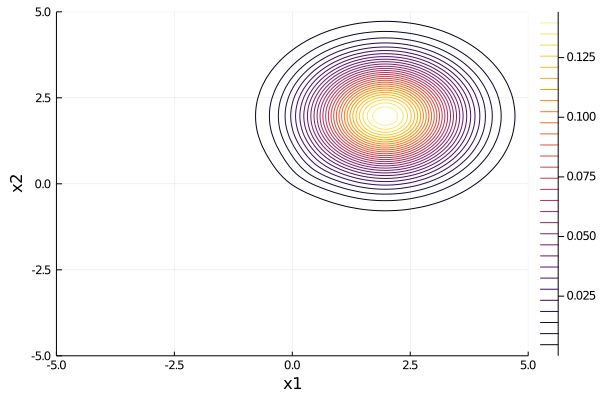
\includegraphics[width=1\linewidth]{../../plot/approx_post_far.png}
\caption{Variational boosting approximating with two components}
\end{subfigure}
\caption{Comparing the target distribution and the variational boosting approximation using the weighed EM component initialization.}
\end{figure}

\begin{figure}[H]
\centering
\begin{subfigure}{0.45\textwidth}
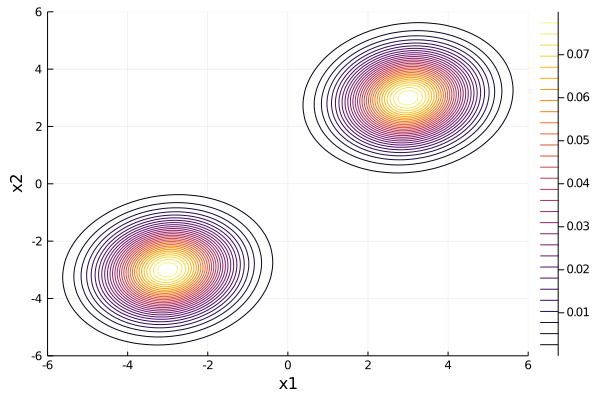
\includegraphics[width=1\linewidth]{../../plot/true_post_close.png}
\caption{True posterior distritbution}
\end{subfigure}
\begin{subfigure}{0.45\textwidth}
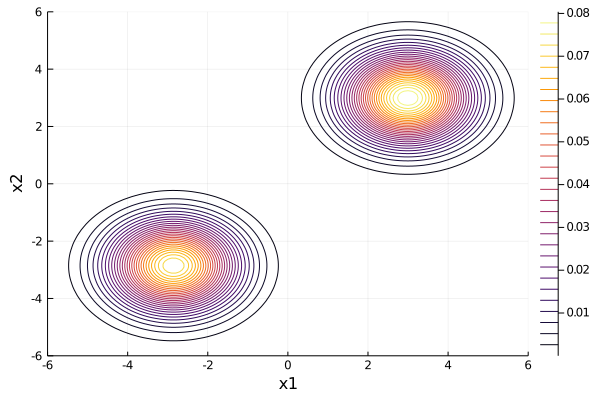
\includegraphics[width=1\linewidth]{../../plot/approx_post_close.png}
\caption{Variational boosting approximating with two components}
\end{subfigure}
\caption{Comparing the target distribution and the variational boosting approximation without the weighed EM component initialization.}
\end{figure}
% ...